\begin{frame}
\frametitle{Ausblick}

\only<1,4,6,9> {
	\begin{itemize}
		\item<1->	Negative Gewichte \onslide<3->{ (Kruskal) }
		\item<4-> 	Computernetzwerke und Steiner-Bäume
		\item<6->	Traveling-Salesman-Problem \onslide<8->{ (Approximation) }
	\end{itemize}
}

\only<2> {
\begin{figure}
		\begin{tikzpicture}[scale=1.6, auto,swap]
    % Draw a 7,11 network
    % First we draw the vertices
    \foreach \pos/\name in {{(0,0)/a}, {(1,1)/b}, {(3,1)/c},
                            {(0,-2)/d}, {(2,0)/e}, {(1,-1)/f}, {(3,-1)/g}}
        \node[vertex] (\name) at \pos {$\name$};
    % Connect vertices with edges and draw weights
    \foreach \source/ \dest /\weight in {b/a/1, c/b/-2,d/a/4,d/b/-9,
                                         e/b/-3, e/c/42, d/g/15,
                                         f/d/4,f/e/7,
                                         g/e/3,g/f/-5}
        \path[edge] (\source) -- node[font=\small] {$\weight$} (\dest);
    
     
    
\end{tikzpicture}
	\caption{Graph mit negativen Gewichten}
	\end{figure}
}

\only<3> {
	\begin{figure}
		\begin{tikzpicture}[scale=1.6, auto,swap]
    % Draw a 7,11 network
    % First we draw the vertices
    \foreach \pos/\name in {{(0,0)/a}, {(1,1)/b}, {(3,1)/c},
                            {(0,-2)/d}, {(2,0)/e}, {(1,-1)/f}, {(3,-1)/g}}
        \node[vertex] (\name) at \pos {$\name$};
    % Connect vertices with edges and draw weights
    \foreach \source/ \dest /\weight in {b/a/1, c/b/-2,d/a/4,d/b/-9,
                                         e/b/-3, e/c/42, d/g/15,
                                         f/d/4,f/e/7,
                                         g/e/3,g/f/-5}
        \path[edge] (\source) -- node[font=\small] {$\weight$} (\dest);
    
     \begin{pgfonlayer}{background}
        \foreach \source / \dest in {b/a,b/c,b/e,b/d,f/g,g/e}
            \path[selected edge] (\source.center) -- (\dest.center);
            
    \end{pgfonlayer}
    
\end{tikzpicture}
	\caption{Graph mit negativen Gewichten}
	\end{figure}
}




\only<5> 	{
					\begin{columns}
						\column{0.5\textwidth}
							\begin{figure}
								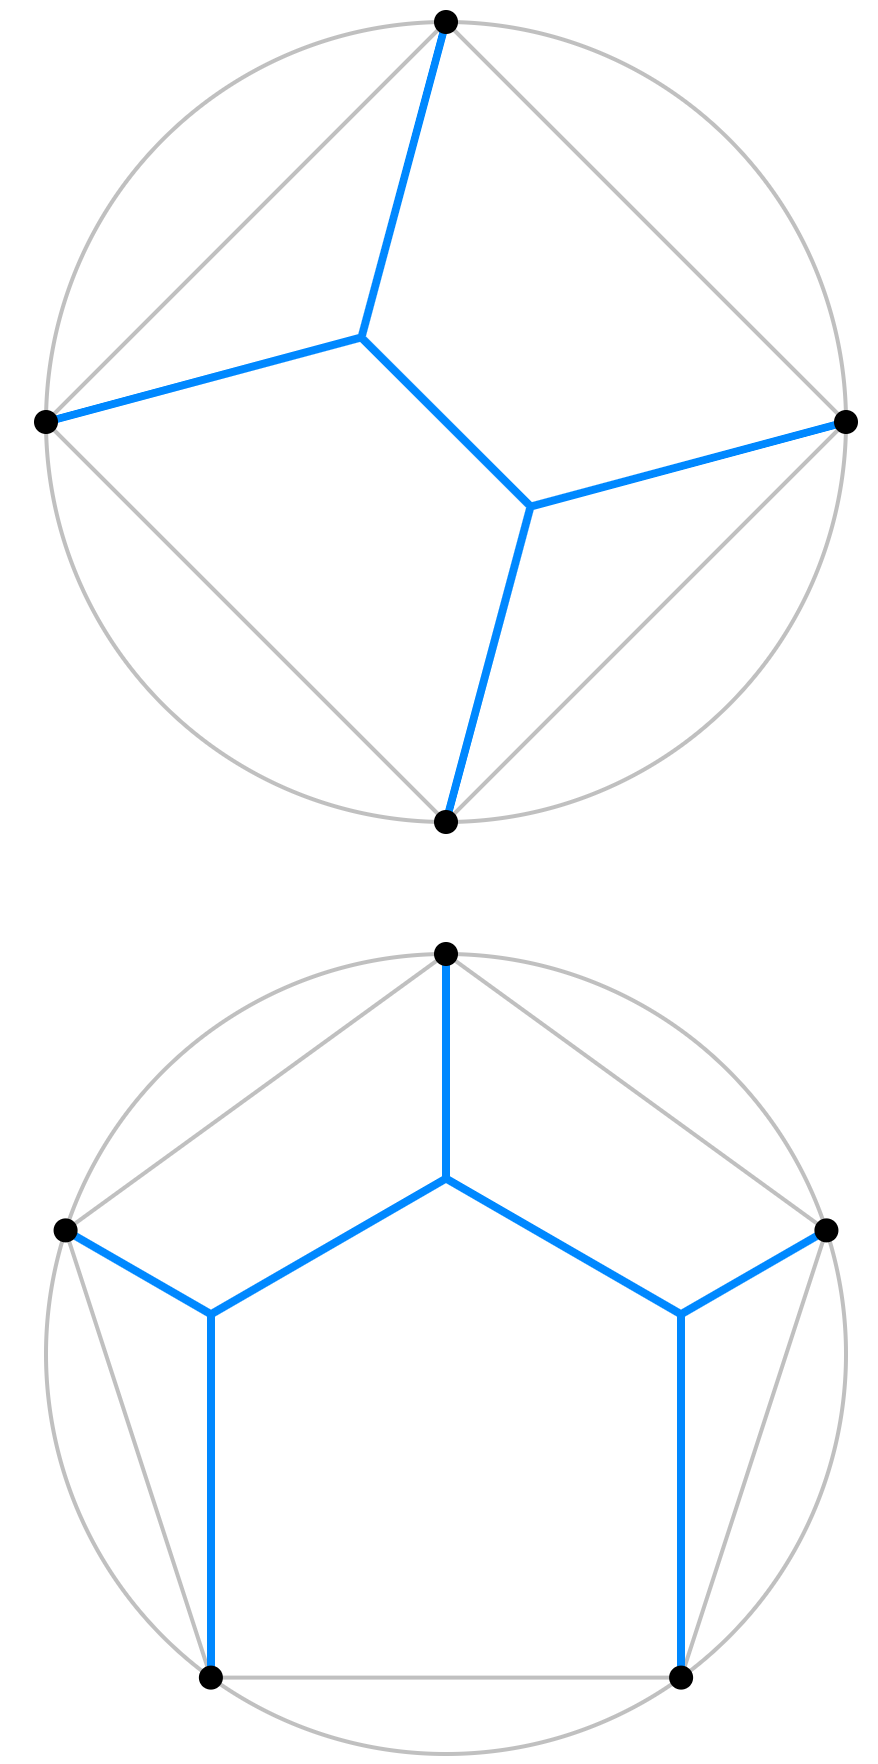
\includegraphics[scale=0.2]{pictures/euclidean-steiner-trees}
								\caption{[Abb2] Steiner Bäume}
							\end{figure}
						\column{0.5\textwidth}
							\begin{figure}
								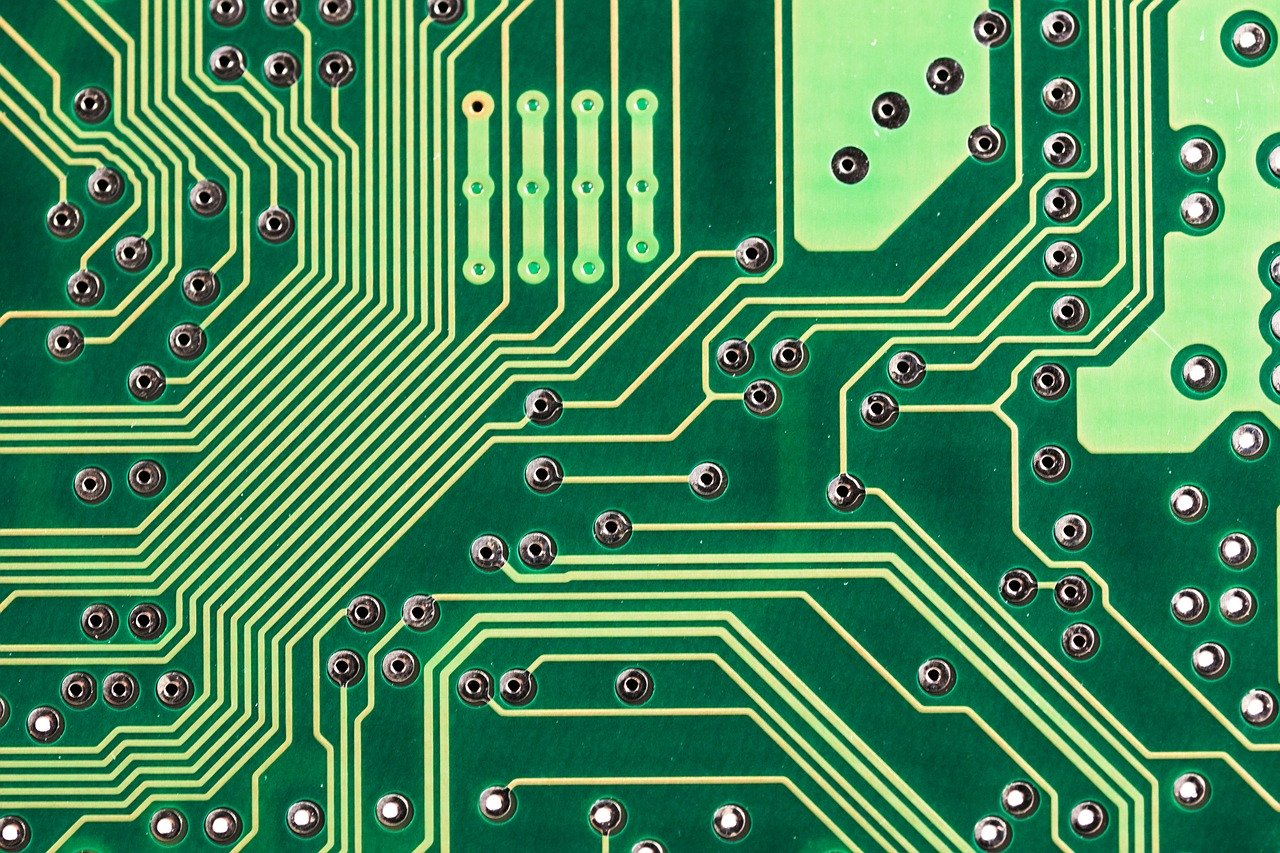
\includegraphics[scale=0.12]{pictures/computer-chip}
								\caption{[Abb3] Computerchip Platine}
							\end{figure}
						\end{columns}
				}

\only<7>	{
					\begin{figure}
						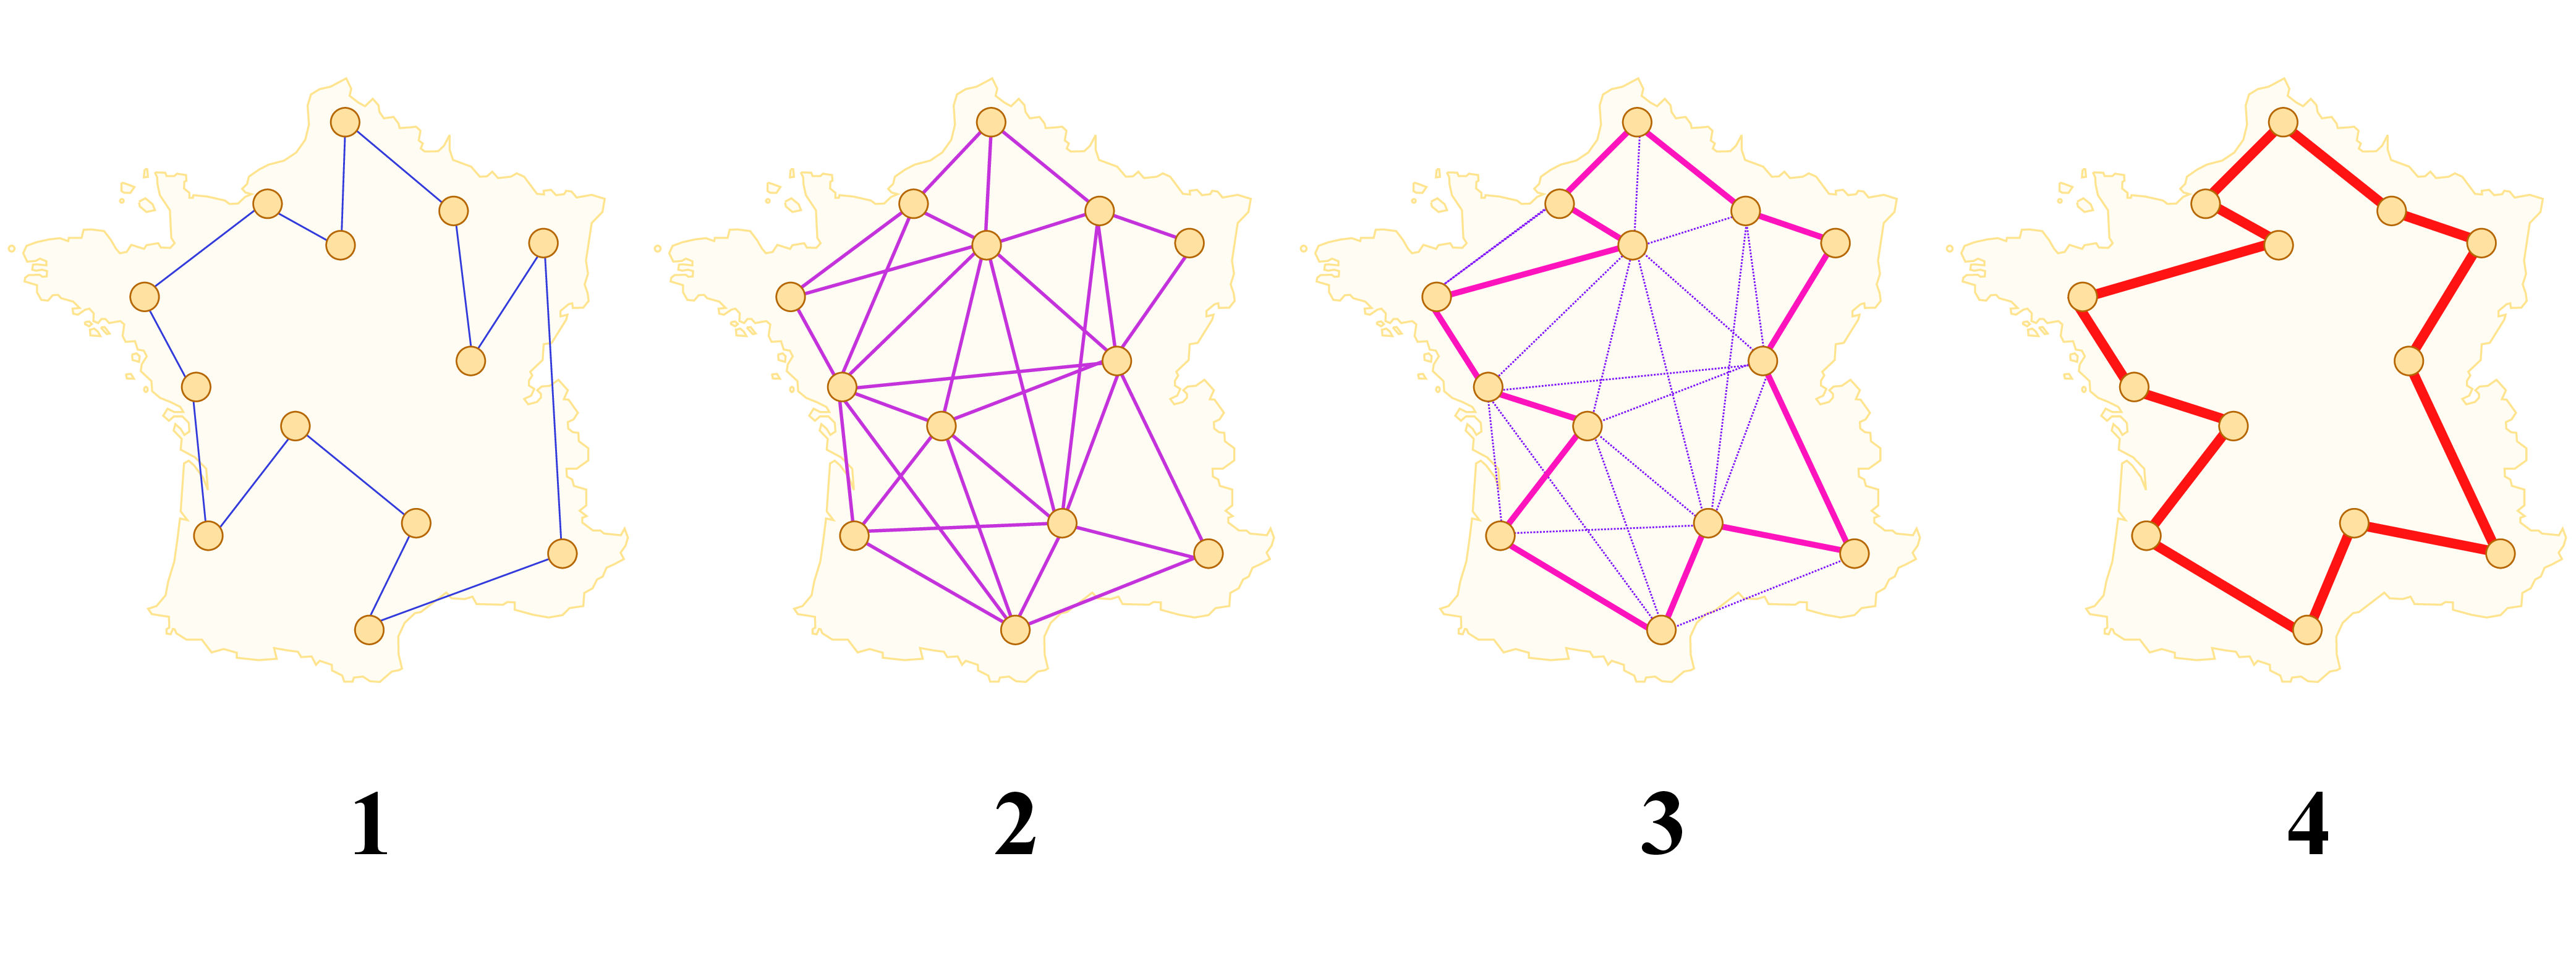
\includegraphics[scale=0.3]{pictures/traveling-salesman-problem}
						\caption{[Abb6] Traveling-Salesman-Problem}
					\end{figure}
				}

\only<8>{
					\begin{figure}
						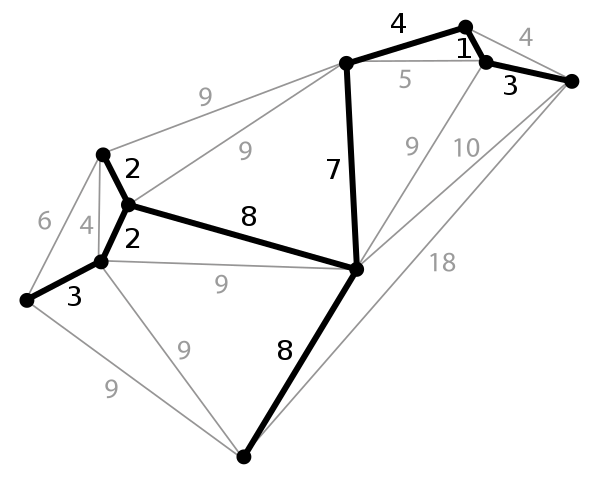
\includegraphics[scale=0.3]{pictures/tsp-msp}
						\caption{[Abb7] Traveling-Salesman-Problem}
					\end{figure}

}

\end{frame}